
\chapter{Methodology}
\begin{refsection}
 
This chapter presents the systematic methodology that was employed to develop and evaluate the Retrieval-Augmented Generation (RAG)-based Large Language Model (LLM) chatbot system for literature search and thesis retrieval in the CSPC Library. The methodology includes the research design, theoretical and mathematical framework, software and hardware tools, instruments, procedures, evaluation metrics, and a conceptual framework.

\section{Research Design}

This study adopted a \textit{constructive research approach}, which focuses on designing and building technological artifacts to address real-world problems and evaluating their practical utility \citeauthor{lukka2003cons} \citeyear{lukka2003cons}. This methodology is particularly well-suited to fields like information systems and artificial intelligence, where the goal is not only theoretical insight but also the creation of innovative, functional systems.

In this research, the primary artifact was a \textit{Retrieval-Augmented Generation (RAG)}-based chatbot integrated with a \textit{Large Language Model (LLM)}. The system is designed to streamline thesis and literature retrieval within the CSPC Library by enabling semantically meaningful interactions between students and academic documents. 

The system incorporated the functionalities of:

\begin{samepage}
\begin{itemize}
    \item CSPC email authentication for user verification
    \item Semantic search using vector embeddings
    \item Query history tracking for improved user experience
    \item Retraining support to adapt to future academic datasets
\end{itemize}
\end{samepage}


These features highlight the system's real-world relevance, sustainability, and potential for long-term utility \cite{hevner2004design}.

The system was developed using Streamlit, which allows rapid deployment of an interactive user interface. The backend combines vector databases and state-of-the-art LLMs, demonstrating how retrieval and generation components can be effectively integrated to improve access to academic resources.

\section{Theorems, Algorithms, and Mathematical Models}

This study implemented advanced machine learning techniques, natural language processing (NLP) models, and the Retrieval-Augmented Generation (RAG) pipeline, integrated with a Large Language Model (LLM) and a vector database. These components collaboratively enabled efficient information retrieval and generation in the context of literature and thesis search within the CSPC Library.

\newpage
\clearpage
\subsection{Retrieval-Augmented Generation (RAG) Pipeline}

The Retrieval-Augmented Generation (RAG) pipeline is a hybrid architecture that combines information retrieval with natural language generation. It allows LLMs to access external documents during inference, thereby improving both accuracy and contextual relevance.

\begin{figure}[htbp]
    \centering
    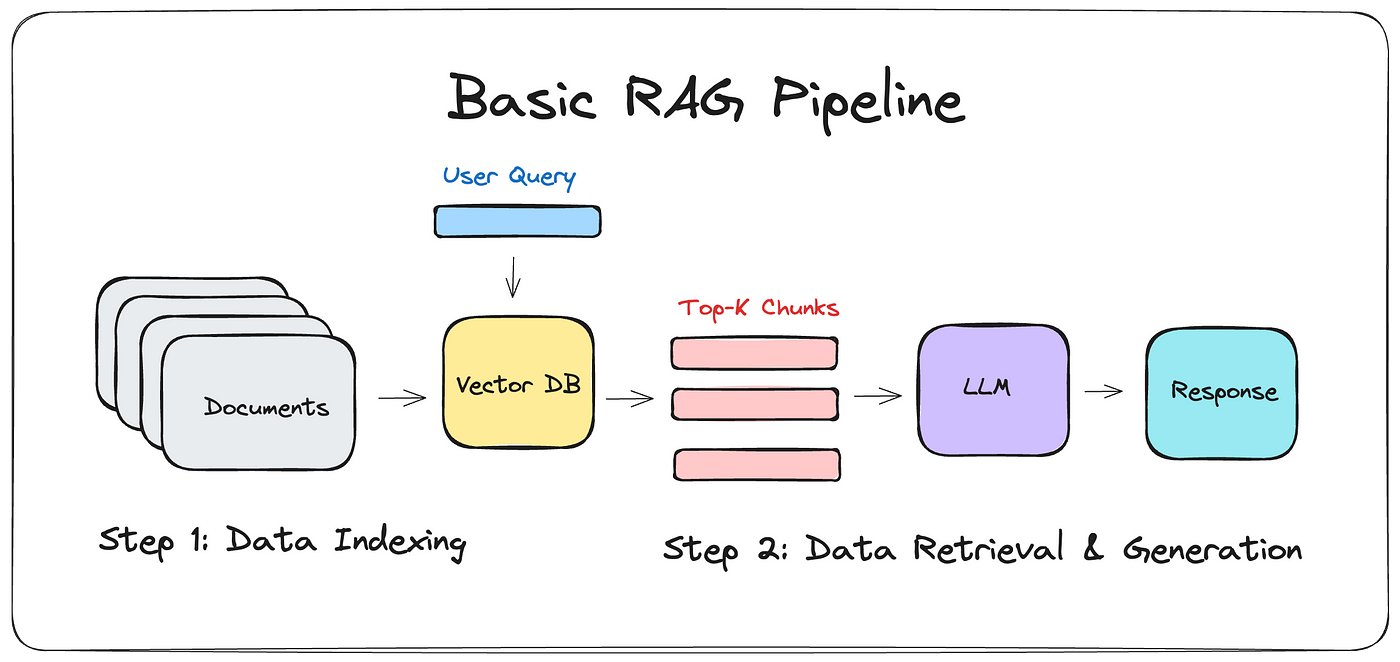
\includegraphics[width=0.7\textwidth]{figures/rag.png}
    \caption{Basic RAG Pipeline by Dr. Julija}
    \label{fig:rag}
\end{figure}

The chatbot’s RAG pipeline, as illustrated in Figure~\ref{fig:rag}, consists of the following key stages:

\subsubsection*{A. Data Indexing}
\begin{itemize}
    \item \textbf{Document Preparation} – Thesis documents were collected and preprocessed into smaller, semantically coherent chunks.
    \item \textbf{Embedding Generation} – Each chunk was converted into a dense vector using a transformer-based embedding model.
    \item \textbf{Vector Database Integration} – These vectors were stored in a vector database (e.g., FAISS) to enable efficient similarity search.
\end{itemize}

\subsubsection*{B. Retrieval and Generation}
\begin{itemize}
    \item \textbf{Query Processing} – When a user submits a query, it will be embedded into a vector representation using the Gemini embedding model (gemini-embedding-001).
    \item \textbf{Similarity Matching} – The system will retrieve the top-K most semantically similar document chunks using cosine similarity.
    \item \textbf{Contextual Generation} – The retrieved chunks will be passed to the Gemini 2.5-flash language model as context, and the model will generate a relevant, factual response.
\end{itemize}


\subsection{Large Language Model}

Large Language Models (LLMs) are cutting-edge artificial intelligence systems capable of processing and generating coherent text. These models are built on advanced neural architectures, trained on massive corpora, and have demonstrated effectiveness across NLP tasks such as summarization, question answering, information retrieval, and dialogue systems \citeauthor{naveed2024} \citeyear{naveed2024}. In this study, the system used the Gemini 2.5-flash LLM to synthesize retrieved academic content with its internal knowledge to generate responses tailored to user queries.


\subsubsection*{Gemini 2.5-flash}

The LLM that was utilized in this project is \textbf{Gemini 2.5-flash}, a model designed for high accuracy and efficiency in natural language understanding and generation. Gemini 2.5-flash is optimized for real-time applications and excels at providing factually accurate, contextually relevant responses. The system integrated this pre-trained model into the RAG framework to augment domain-specific information retrieval for CSPC Library users.

\section{Materials and Statistical Tools}

To ensure optimal performance of the RAG-based LLM system, several key hardware and software components are required.

\subsubsection*{Hardware}
\begin{table}[H]
    \centering
    \caption{Hardware Requirements}
    \label{tab:hardware_requirements}
    \begin{tabular}{ll}
        \hline
        \textbf{Component}       & \textbf{Specification}                     \\ \hline
        Processor (CPU)          & Modern Multi-core CPU                      \\
        Memory (RAM)             & 16 GB or higher                            \\
        Storage                  & 1 TB SSD or higher                         \\
        Graphics Card (GPU)      & NVIDIA RTX 3090+ (recommended)             \\
        \hline
    \end{tabular}
\end{table}

A modern multi-core CPU enables efficient data processing and model inference, ensuring smooth query execution. At least 16 GB of RAM is recommended to manage large-scale embeddings and real-time retrieval operations effectively. 

A 1 TB SSD is preferred due to its high read/write speeds, which significantly enhance data indexing and retrieval. Given the resource-intensive nature of embedding computations and AI-driven text generation, a high-performance GPU, such as an NVIDIA RTX 3090 or better, is crucial for accelerating deep learning inference and vector operations.


\subsubsection*{Software}

\begin{table}[H]
    \centering
    \caption{Software Requirements}
    \label{tab:software_requirements}
    \begin{tabular}{ll}
        \hline
        \textbf{Component}              & \textbf{Specification}                        \\ \hline
        Programming Language            & Python 3.10+                                  \\
        Vector Database                 & e.g. FAISS                                         \\
        Language Model                  & Gemini 2.5-flash                                       \\
        Embedding Model                 & gemini-embedding-001                            \\
        Web Framework                   & Streamlit                                     \\
        Libraries                       & \begin{tabular}[c]{@{}l@{}}LangChain\\ PyMuPDF\\ NumPy\\ PyPDFLoader\end{tabular}   \\
        \hline
    \end{tabular}
\end{table}

Python 3.10 or later serves as the core programming language due to its comprehensive support for machine learning and natural language processing. FAISS is used as the vector database to facilitate fast and accurate semantic search. The system leverages Gemini 2.5-flash (deployed locally via Ollama) as its LLM, which ensures data privacy during query generation. Gemini-embedding-001 transforms preprocessed text chunks into semantically rich vector representations. The Streamlit framework is used to build an interactive user interface, allowing seamless user interactions.

Document parsing and extraction are managed through the PyMuPDF library, ensuring accurate and efficient retrieval of textual data from PDF files. NumPy supports numerical operations, while LangChain manages the orchestration of LLMs during query interpretation and response generation.

\section{Instruments}


The instruments utilized in this study included a curated dataset, a vector database, a user evaluation questionnaire, and an automated evaluation toolkit. The dataset consisted of all available PDF thesis documents sourced from the CSPC Library, which were parsed using the PyMuPDF library for text extraction. These documents underwent preprocessing, including cleaning and segmentation into manageable chunks, before being embedded using \textit{gemini-embedding-001}, a modern embedding model known for its semantic richness and high compatibility with retrieval tasks.


The vectorized representations of these chunks were then stored in \textit{FAISS}, an open-source vector database optimized for fast similarity search and retrieval, which was vital for the implementation of the RAGAS framework~\cite{trychroma2023chroma}.

To assess both technical and user-centered performance, multiple evaluation instruments were employed. A user questionnaire was used to gather feedback on usability, accuracy, and overall satisfaction, applying a 5-point Likert scale for consistent measurement.

Additionally, the RAGAS (Retrieval-Augmented Generation Assessment Suite) toolkit was utilized to automatically evaluate the quality of system outputs using metrics such as \textbf{context precision}, \textbf{faithfulness}, and \textbf{answer relevance}~\cite{shinn2023ragas}. These instruments ensured a rigorous and balanced evaluation of the proposed system from both system-level and user perspectives~ \cite{lin2021bert}.

\section{Statistical Tools}

The evaluation of the system incorporated both descriptive and inferential statistical tools. Descriptive statistics such as \textit{mean} and \textit{standard deviation} summarized user feedback, providing insight into central tendencies and variability in user experience~\cite{holmes2023chatbot}.

Additionally, \textbf{Cronbach’s Alpha} was used to assess the internal consistency and reliability of the usability survey instrument. This coefficient measured whether the questionnaire items consistently reflected the intended construct of system usability, ensuring the validity of user feedback.

Finally, the RAGAS framework was applied to evaluate the system's technical performance. It included metrics such as \textit{context precision}, \textit{context recall}, and \textit{faithfulness}. These metrics assessed how accurately the system retrieved and utilized relevant documents to generate responses~\cite{holmes2023chatbot, ameli2024ranking, lin2024satisfaction}.

\section{Procedures}

The procedures encompassed the collection and preprocessing of academic data, vector-based indexing, retrieval using semantic search, LLM-based response generation, and multi-metric evaluation using RAGAS.

Each stage was designed to ensure the integrity, replicability, and effectiveness of the system in addressing the research objectives. By detailing the technical and methodological steps, this section served as a transparent and structured guide for future researchers seeking to replicate or build upon this study.

\subsection*{Data Collection}
PDF thesis documents were gathered from CSPC Library’s digital archives, focusing on undergraduate theses and institutional research. The collection process ensured that documents were academically relevant and representative of typical user queries.

\subsection*{Data Preprocessing}
\begin{itemize}
    \item \textbf{Text Extraction:} PyMuPDF will be used to convert PDF files into structured plain text.
    \item \textbf{Cleaning:} Non-informative characters and formatting will be removed.
    \item \textbf{Text Chunking:} Text will be segmented into manageable chunks to enhance semantic search accuracy.
\end{itemize}

\subsection*{Indexing and Vector Embedding}
\begin{itemize}
    \item \textbf{Vector Embedding:} Each text chunk will be embedded using gemini-embedding-001.
    \item \textbf{Database Construction:} FAISS will store the vectorized content along with metadata such as document titles, authors, and section headers.
\end{itemize}

\subsection*{Query Handling and Semantic Retrieval}
\begin{itemize}
    \item \textbf{Query Encoding:} The user’s natural language query will be encoded using the same embedding model.
    \item \textbf{Similarity Search:} The encoded query will be matched with stored vectors to retrieve the top-K relevant chunks.
\end{itemize}

\subsection*{Augmented Input Generation}
The retrieved chunks will be concatenated with the user query to create an augmented prompt, providing contextual grounding for accurate response generation.

\subsection*{Response Generation}
The Gemini 2.5-flash language model will process the augmented input to generate a response that is factually aligned with the source documents.

\subsection*{Output Presentation}
The system will display the generated response via a user interface that includes metadata such as the source thesis title and section, encouraging transparency and academic integrity.

\subsection*{Performance Evaluation}
\begin{itemize}
    \item \textbf{Automated Evaluation:} Metrics from the RAGAS framework, Context Precision, Context Recall, and Faithfulness, will be calculated.
    \item \textbf{Human Evaluation:} A usability questionnaire was distributed to a sample of student users to assess the system’s clarity, ease of use, and usefulness in retrieving academic information.
\end{itemize}

\section{Evaluation Metrics}

\hspace{0.4cm}The researchers used a framework called \textbf{RAGAS} that comprised specific metrics to assess Retrieval-Augmented Generation (RAG)-based architectures, thereby ensuring precise measurements of both retrieval quality and generation fidelity~\cite{oubah2024advanced}. This framework evaluated the model's performance using the following metrics: \textbf{Context Precision}, \textbf{Context Recall}, and \textbf{Faithfulness}. Each metric was essential in addressing the system’s retrieval and generation performance.

\subsection*{Context Precision}

The Context Precision metric was used to evaluate the retrieval quality of the RAG chatbot within the CSPC Library. It measured the proportion of relevant document chunks among the top $K$ retrieved results, emphasizing the system's ability to present highly relevant content at higher ranks. A higher Context Precision indicated that the system effectively prioritized relevant information for the user.

\begin{equation}
\centering
\text{Context Precision@K} = 
\frac{
    \sum_{k=1}^{K} \left( \text{Precision@k} \times v_k \right)
}{
    \text{Total number of relevant items in the top } K \text{ results}
}
\end{equation}

where $\text{Precision@k}$ is the precision at rank $k$, and $v_k$ is a binary indicator variable such that $v_k = 1$ if the chunk at position $k$ is relevant, and $v_k = 0$ otherwise. Here, $K$ indicates the cutoff for the top results evaluated. The denominator normalizes the metric by accounting for the total number of relevant items within the top $K$ retrieved results. This weighted approach ensures that relevant items retrieved earlier in the ranking contribute more significantly to the final score, making the metric especially meaningful for library retrieval tasks.

The precision at each position $k$, denoted as Precision@k, is computed as follows:

\begin{equation}
\centering
\text{Precision@k} = 
\frac{
    \text{true positives@k}
}{
    \text{true positives@k} + \text{false positives@k}
}
\end{equation}

where $\text{true positives@k}$ is the number of relevant chunks retrieved up to position $k$, and $\text{false positives@k}$ is the number of non-relevant chunks retrieved up to the same position. This component metric quantifies retrieval accuracy at each rank and serves as a foundation for the overall Context Precision@K calculation.

\newpage
\clearpage
\subsection*{Context Recall}

Context Recall was used to evaluate the comprehensiveness of the retrieval system in capturing all relevant information necessary to answer a query. It measured the proportion of relevant chunks successfully retrieved by the RAG chatbot within the CSPC Library, ensuring minimal omission of important academic content.

\begin{equation}
\centering
\text{Context Recall} = \frac{\text{Number of relevant claims supported by retrieved chunks}}{\text{Total number of relevant claims in the reference answer}}
\end{equation}

where:
\begin{itemize}
    \item \textit{Number of relevant claims supported by retrieved chunks} refers to the count of factual claims in the ground truth answer that can be attributed to the retrieved document chunks,
    \item \textit{Total number of relevant claims in the reference answer} represents all the factual claims present in the ground truth answer that ideally should be covered by the retrieval process.
\end{itemize}

This metric captures how effectively the system covers the necessary knowledge, with a value ranging between 0 and 1, where 1 indicates perfect recall. It ensures that critical academic information is not missed during retrieval, making it an essential part of evaluating the RAG chatbot system.

\newpage
\clearpage
\subsection*{Response Relevance}

Response Relevance was a critical metric used to evaluate how well the RAG chatbot's generated answer addressed the specific query posed by users in the CSPC Library. This metric ensured that the chatbot provided focused, comprehensive, and directly applicable responses to academic inquiries, minimizing irrelevant or incomplete information that could hinder research efficiency.

\begin{equation}
\centering
\text{Response Relevance} = \frac{1}{N} \sum_{i=1}^{N} \cos(E_{g_i}, E_o)
\end{equation}

where:
\begin{itemize}
    \item $N$ is the number of artificially generated questions based on the response (typically 3),
    \item $E_{g_i}$ is the embedding of the $i$-th generated question derived from the response,
    \item $E_o$ is the embedding of the original user query,
    \item $\cos(E_{g_i}, E_o)$ represents the cosine similarity between the generated question embedding and the original query embedding.
\end{itemize}

This metric works on the idea that if the chatbot's response sufficiently answers the original query, then questions generated from that response will semantically align with the original question, this involves generating multiple artificial questions, embedding both the response-generated questions and the original query into vector representations, and calculating the mean cosine similarity to measure alignment, which ensures that the retrieved academic information closely matches the research needs of CSPC Library users.

\newpage
\clearpage
\subsection*{Faithfulness}

Faithfulness is a critical metric for evaluating the factual consistency of the RAG chatbot's generated responses with respect to the retrieved context from the CSPC Library. This metric ensures that all claims made in the chatbot's answer are directly supported by the information present in the retrieved documents, thereby minimizing hallucinations and maintaining academic integrity.

\begin{equation}
\centering
\text{Faithfulness} = \frac{\text{Number of claims in the response supported by retrieved context}}{\text{Total number of claims in the response}}
\end{equation}

where:
\begin{itemize}
\item \textit{Number of claims in the response supported by retrieved context} refers to the count of factual statements in the generated answer that can be directly verified or inferred from the retrieved context chunks,
\item \textit{Total number of claims in the response} is the complete count of all factual statements made in the answer, regardless of whether they are supported by the context.
\end{itemize}

A faithfulness score of $1.0$ indicates that all claims in the response are grounded in the retrieved context, while lower scores reveal the presence of unsupported or hallucinated information. In the context of academic literature search and thesis retrieval, maintaining high faithfulness is essential to ensure that the chatbot's answers are trustworthy and factually accurate, directly reflecting the content of the CSPC Library's resources.


\newpage
\clearpage
\section{Conceptual Framework}

The conceptual framework served as the foundational blueprint for the RAG-based chatbot system. It emphasized the end-to-end interaction of modules required to support intelligent, accurate, and efficient academic document retrieval. As illustrated in Figure~\ref{fig:conceptual_framework}, the system followed a cyclical process beginning with data collection and ending with system evaluation and refinement.
In Figure~\ref{fig:conceptual_framework}, the arrows were used solely to visually indicate the step-by-step flow of each component within the chatbot framework; they did not signify any technical operation or special relationship beyond showing the direction of the process. 

This visualization helps guide readers through the sequence of the system stages, ensuring clarity at the outset.

\begin{figure}[H]
    \centering
    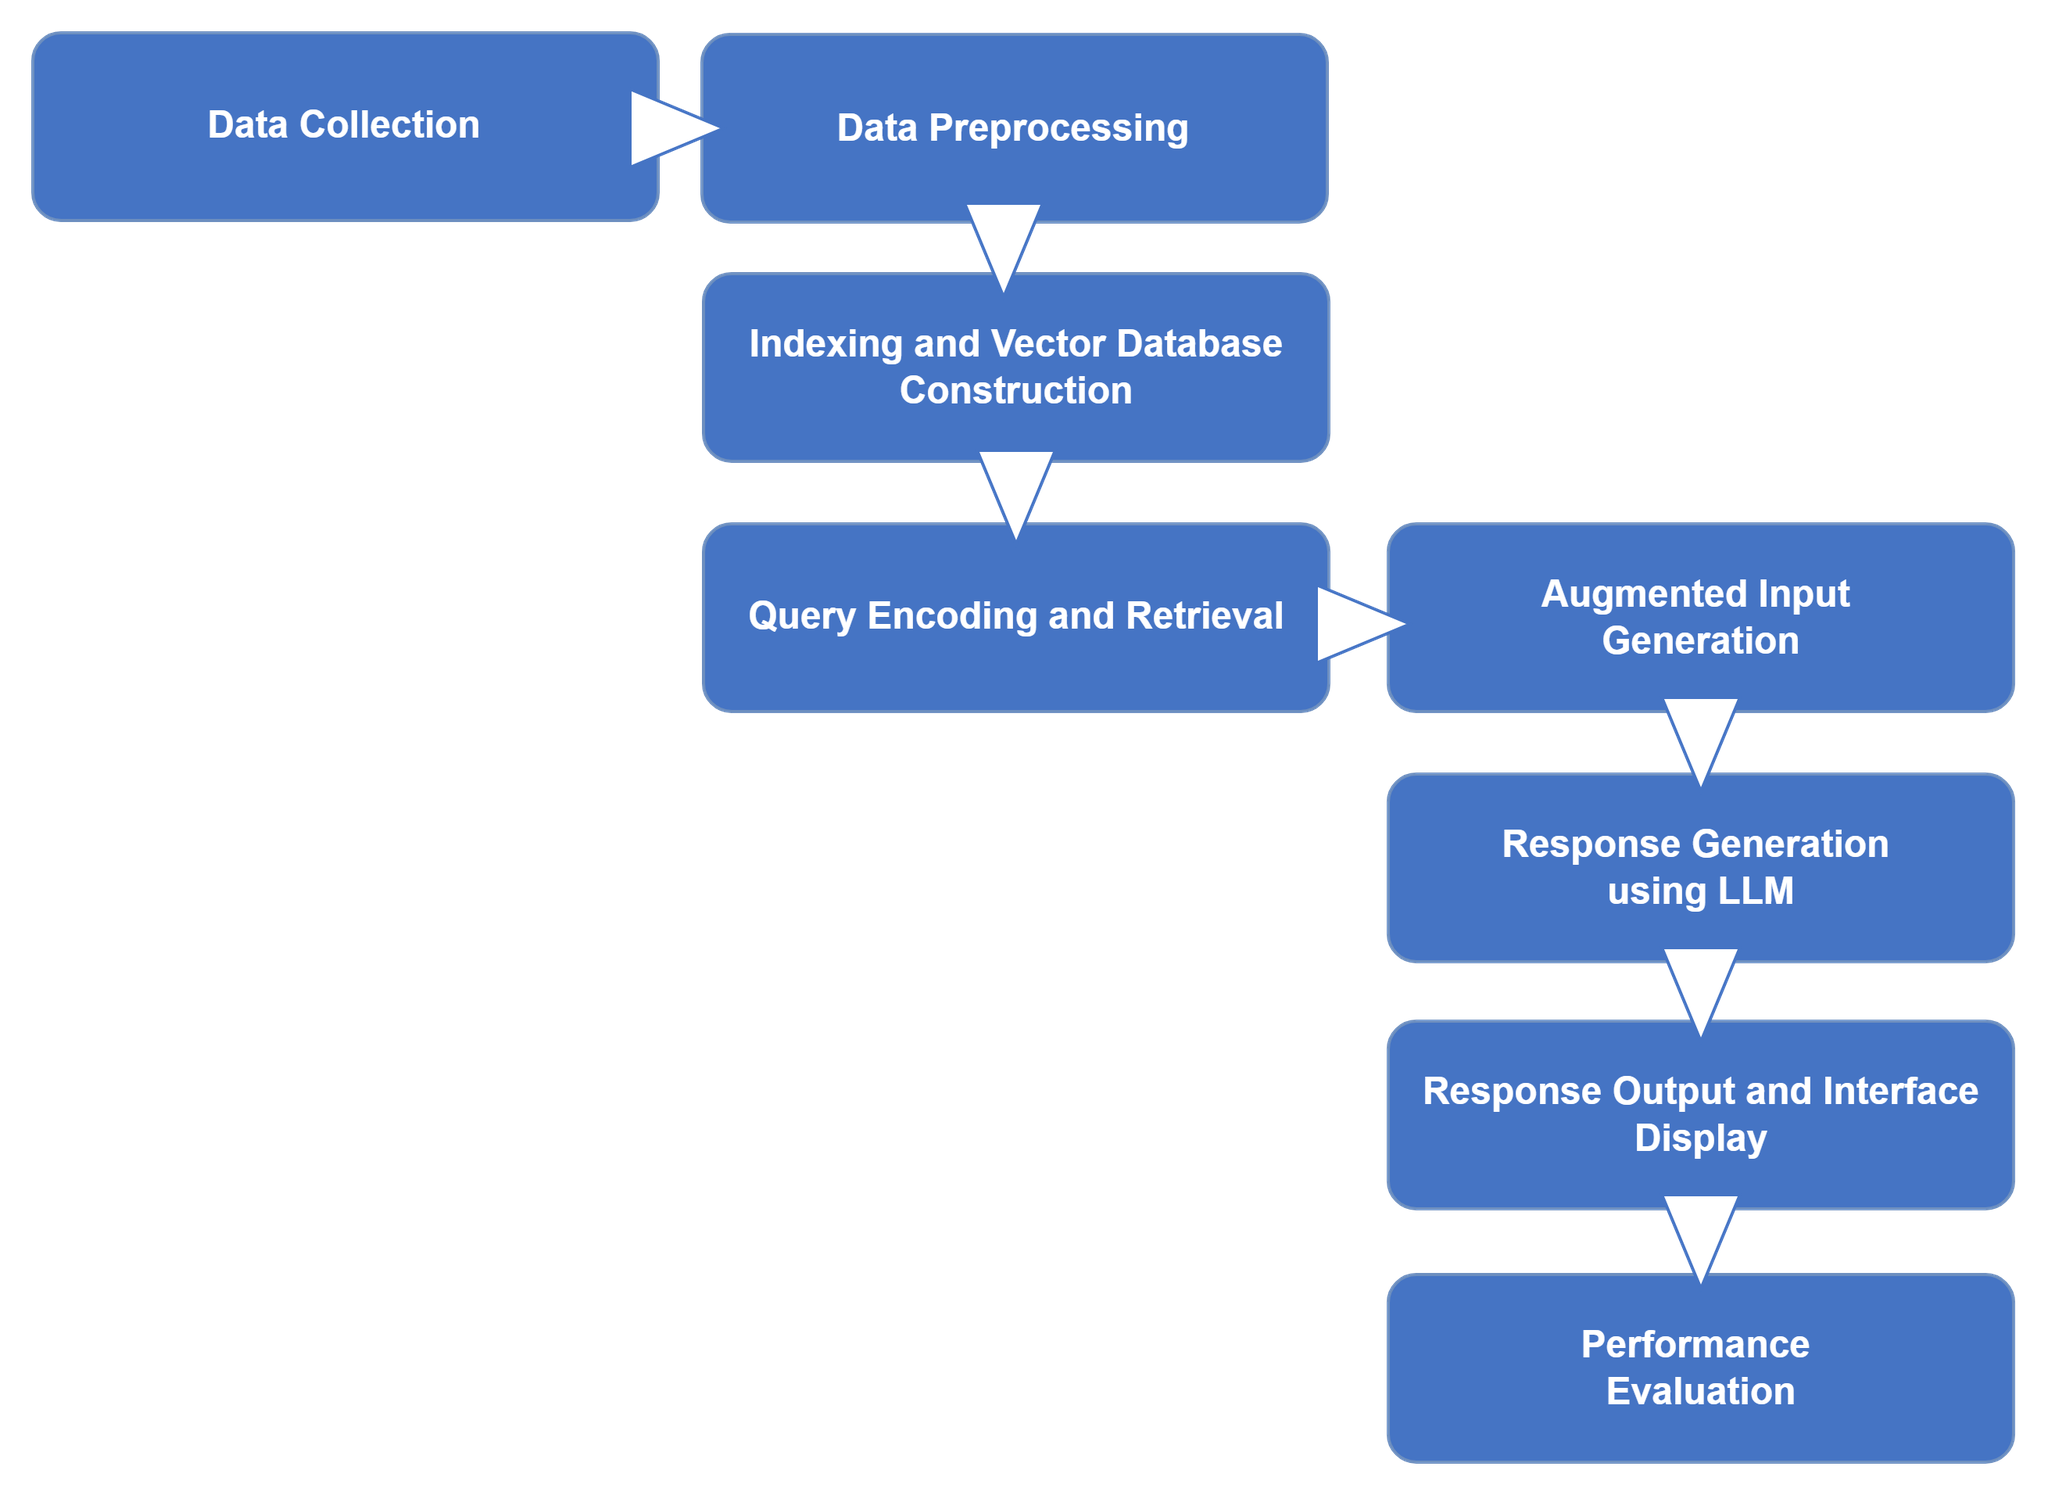
\includegraphics[width=0.7\textwidth]{figures/framework.png}
    \caption{Conceptual Framework of the RAG-Based Chatbot System}
    \label{fig:conceptual_framework}
\end{figure}

The process began with \textbf{data collection}, where PDF-format academic documents such as undergraduate theses and institutional research papers were sourced from the CSPC Library’s digital repository. These documents formed the primary knowledge base of the system.

In the \textbf{data pre-processing} phase, tools like PyMuPDF were used to extract plain text from the collected PDFs. The extracted content underwent cleaning and normalization to remove non-informative characters, followed by segmentation into semantically meaningful text chunks.

Next, the system performed \textbf{model training}, where embedding models such as gemini embeddings were used to transform the text chunks into vector representations.


These embeddings preserved the semantic meaning of the documents and prepared them for storage and retrieval.

The \textbf{input sampling} stage supported the gathering and simulation of user queries. These sample inputs reflected typical academic inquiries posed by students when searching for specific thesis content.

In the \textbf{input pre-processing} phase, user queries were tokenized and encoded using the same embedding model applied during training. This enabled semantic similarity comparison between the user query and the pre-embedded document vectors.

The system then proceeded to \textbf{location mapping}, which corresponded to the semantic search function performed using FAISS. Here, the system retrieved the top-K most relevant document chunks by measuring vector similarity.

During \textbf{model inference}, an augmented input was created by combining the user query with the retrieved chunks. This augmented prompt was forwarded to a generative language model (e.g., Gemini 2.5-flash) to produce a contextually grounded response aligned with the original academic documents.

Finally, \textbf{performance evaluation} was conducted using a dual-layer assessment. System-level performance was measured using the RAGAS framework with metrics such as Context Precision, Context Recall, and Faithfulness. This framework ensured that each component of the RAG-based chatbot system operated in coordination, contributing to a reliable and academically useful tool for thesis retrieval and literature assistance.

%=======================================================%
%%%%% Do not delete this part %%%%%%
\clearpage

\printbibliography[heading=subbibintoc, title={\centering Notes}]
\end{refsection}
